\chapter{Resultados y Discusión}
\label{resultadosdiscusion}
\ifpdf
  \graphicspath{{Chapter7/Chapter7Figs/PNG/}{Chapter7/Chapter7Figs/PDF/}{Chapter7/Chapter7Figs/}}
\else
  \graphicspath{{Chapter7/Chapter7Figs/EPS/}{Chapter7/Chapter7Figs/}}
\fi

\markboth{\hfill \thechapter. Resultados y Discusión}{\hfill \thechapter. Resultados y Discusión}

\section{Ambiente de Ejecución}

Las pruebas para la obtención de los resultados se ejecutaron en una computadora personal con la siguiente configuración:
\begin{itemize}
   \item Procesador Intel\textcopyright{}  Core\texttrademark{} i5 2.3 GHz.
    \item Memoria RAM de 8 GB. 
    \item Disco SSD de 256 GB.
    \item Sistema Operativo Linux Mint en su version 18.3 Cinnamon 64-bit.
\end{itemize}

% Para la puesta en marcha de la aplicación \textit{TapeYty} lo requerimientos no funcionales son los siguientes:

% \begin{enumerate}
%     \item 
% \end{enumerate}

\section{Resultados Obtenidos}

% En esta sección se presenta un análisis de los resultados obtenidos con \textit{TapeYty}. 

La Figura \ref{fig:RecorridoActualZona83} muestra el camino trazado por el GPS instalado en el vehículo recolector 129 en la zona 83 de trabajo con una distancia total recorrida de 16.940 km, donde se observa que varios segmentos de calles son atravesados repetidas veces mientras que otros dentro de la zona no son atravesados. En la práctica, los recolectores suelen acumular las bolsas de basura de varias casas en una esquina, evitando que el conductor entrase a ciertas calles, lastimosamente no es posible asegurar que dichos segmentos hayan recibido el servicio. Las avenidas de color naranja que delimitan la zona no forman parte de la recolección pero algunos segmentos de estas avenidas son utilizados para poder acceder a las calles que si deben ser cubiertas por el servicio.

\begin{figure}[htbp]
    \centering
    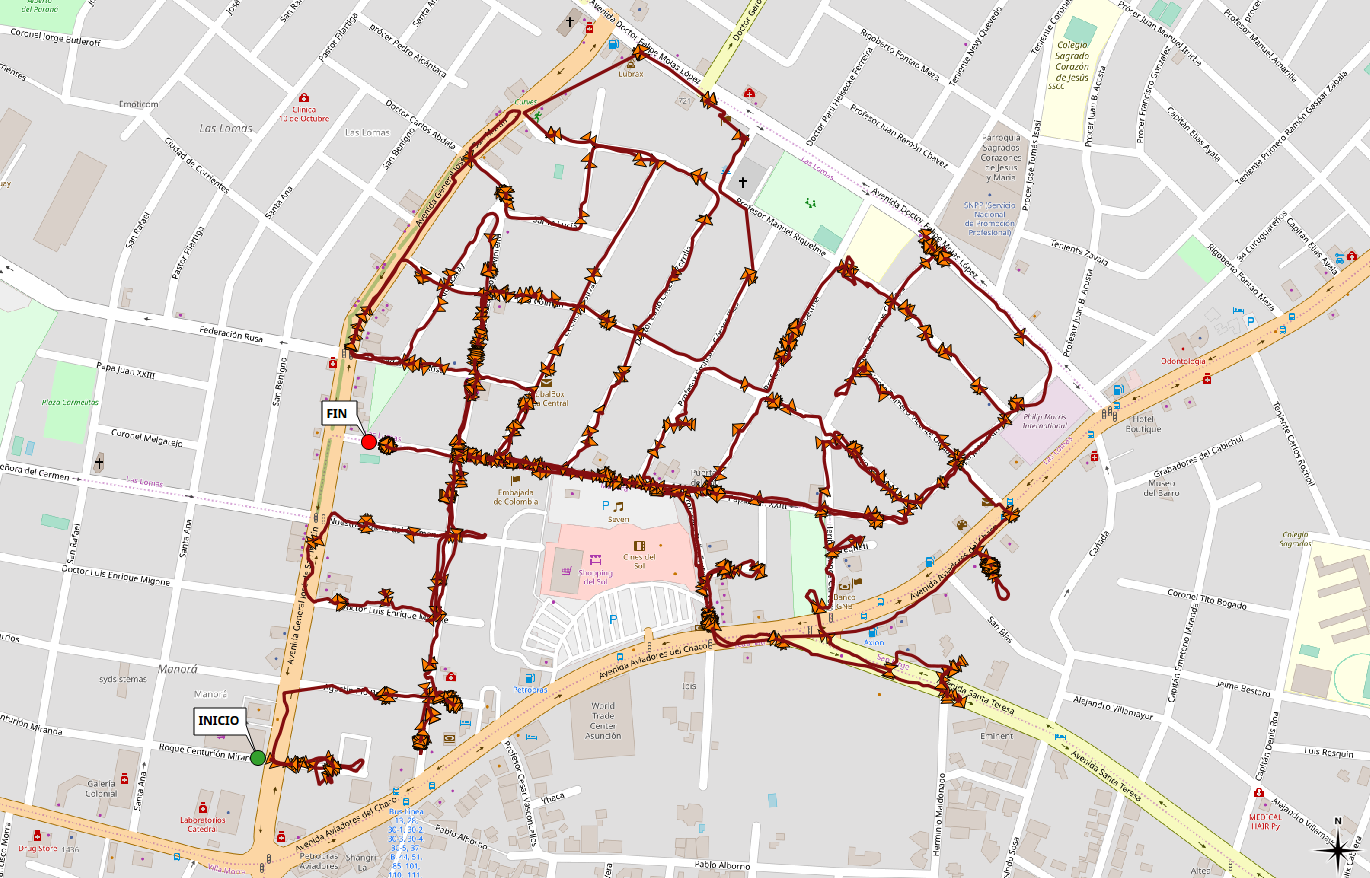
\includegraphics[width=\textwidth]{recorridoActual83.png}
    \caption{Ruta actual. [Fuente: Datos obtenidos en fecha 28/11/2018 del GPS instalado en camión recolector 129 de la DSU]}
    \label{fig:RecorridoActualZona83}
\end{figure}

En la Figura \ref{fig:RecorridoTapeYtyZona83} se muestra el camino generado por \textit{TapeYty} con una cobertura total de las calles que deben ser visitadas en la zona. La secuencia del recorrido se encuentra especificada en los segmentos. La metodología de trabajo se mantiene de acuerdo con lo establecido por la DSU como en la Figura \ref{fig:RecorridoActualZona83}, y por lo tanto, la misma delimitación de zonas.

\begin{figure}[htbp]
    \centering
    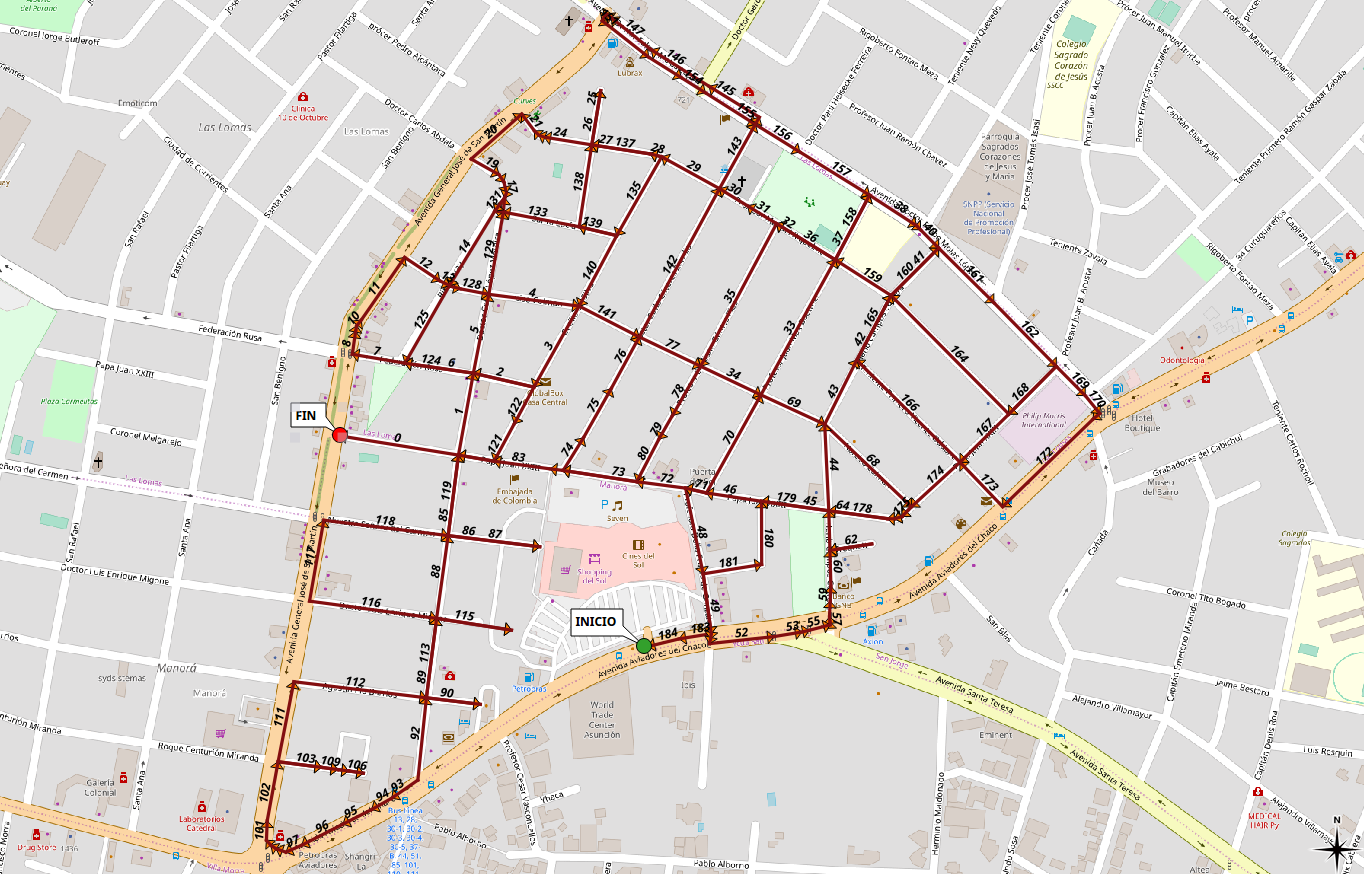
\includegraphics[width=\textwidth]{recorrido83CoberturaTotal.png}
    \caption{Ruta generada por \textit{TapeYty} con cobertura completa.}
    \label{fig:RecorridoTapeYtyZona83}
\end{figure}

Las calles sin salida, las estrechas y las que limitan una zona pero que no deben ser visitadas necesariamente son gestionadas mediante \textit{TapeYty}. Por ejemplo, en la Figura \ref{fig:RecorridoTapeYtyZona83Opcionales} ciertos segmentos de calles pasan a ser opcionales para el paso de camiones simulando el procedimiento llevado a cabo por el equipo de recolección (ver Figura \ref{fig:RecorridoActualZona83}).

% PAPER
% El punto de inicio de la ruta generada se representa en el mapa con un punto verde, el punto final con un punto rojo y la secuencia a seguir se encuentra especificada en los segmentos de calle. Algunos números de secuencia no son visibles en el mapa debido a que los segmentos son muy pequeños y se requiere de acercamiento para verlos, por ejemplo, el sexto segmento a atravesar no es visible debido a su longitud. El sistema permite exportar un archivo con formato GPX (\textit{GPS eXchange Format}) de la ruta generada que es utilizada para la navegación de la ruta.

Algunas zonas cuentan con varios segmentos de calles de un único sentido, y si solo se utilizan los segmentos dentro de la zona, el resultado podría resultar infactible computacionalmente o más costoso en distancia, motivo por el cual se agrega una banda perimetral, tal como en \citet{Braier2017AnArgentina}, de 220 metros representándose a los segmentos de calle dentro de la banda como arcos auxiliares del modelo. Esta situación donde los camiones salen unas cuadras de su zona para volver a entrar es común en la práctica actual de la recolección de residuos.

\begin{figure}[htbp]
    \centering
    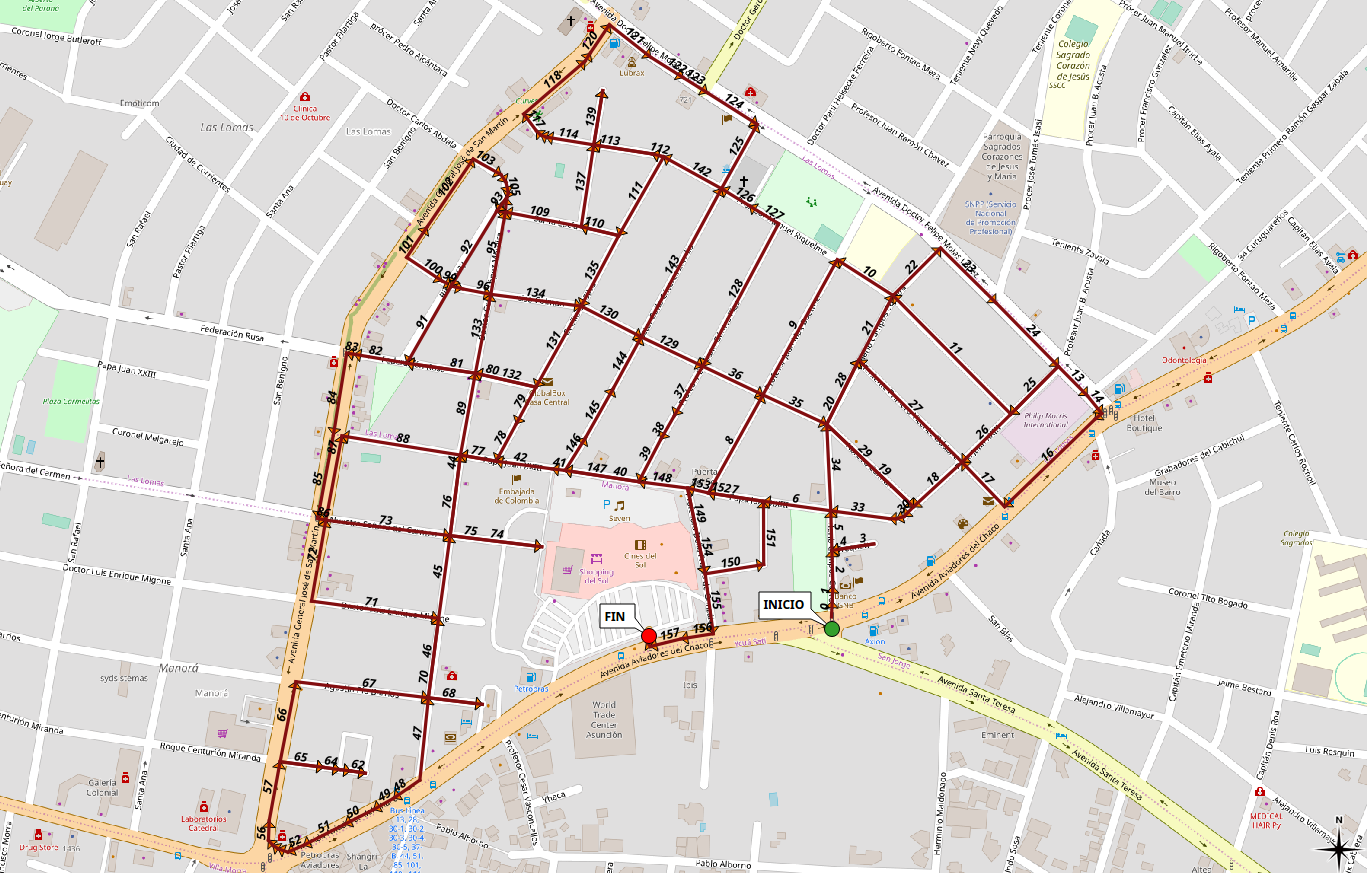
\includegraphics[width=\textwidth]{recorrido83Opcionales.png}
    \caption{Ruta generada por \textit{TapeYty} con segmentos opcionales.}
    \label{fig:RecorridoTapeYtyZona83Opcionales}
\end{figure}

En la Tabla \ref{table:comparacionZona83} se presenta el resultado de la zona 83. En la primera columna se listan las características del modelo: número de iteraciones, los tiempos de ejecución y distancia de la solución. La segunda columna se refiere al escenario en el que todos los segmentos de calles dentro de la zona deben ser visitados por el vehículo recolector y la tercera columna se refiere al escenario en el que 6 segmentos de calles de sentido único y 3 de doble sentido fueron marcados como opcionales desde la aplicación. Si analizamos y comparamos la segunda y tercera columna podemos observar que ambos escenarios coinciden en la cantidad de vértices en el grafo, cantidad de calles de sentido único y de doble sentido, no así en la cantidad de arcos auxiliares debido a la diferencia en la cantidad de segmentos opcionales.

En el primer escenario es posible resolver mediante la técnica de mezcla de subtours recién en la segunda iteración, mientras que en el segundo se puede resolver con la misma técnica ya en la primera iteración. Se observa también que el tiempo de ejecución del modelo es levemente menor para el segundo escenario. Realizar la expansión del grafo a partir de los datos de entrada es el paso que requiere de mayor tiempo en la aplicación. En ambos escenarios se redujo la distancia con respecto al recorrido actual, en el primero en un 20.31\%  y en el segundo un 28.50\%, con 3.44105 km. y 4.82806 km. menos respectivamente.

\begin{table}[htbp]
\caption{Resultados y análisis para la zona 83}
\begin{tabular}{lll}
\hline
\multirow{2}{*}{Zona 83}                            & \multicolumn{2}{l}{Cobertura de segmentos de calles} \\ \cline{2-3} 
                                                    & Sin opcionales           & Con opcionales           \\ \hline
$|V|$                                                   & 1352                     & 1352                     \\
$|E|$                                                   & 420                      & 420                      \\
$|AM|$                                                  & 256                      & 256                      \\
$|Aaux|$                                                & 1567                     & 1579                     \\
Iteraciones                                         & 2                        & 1                        \\
Tiempo de expansión (s)                      & 20.54530                 & 22.06926                 \\ 
Tiempo de ejecución del modelo (s)            & 0.52790                  & 0.31660                  \\ 
Tiempo de secuenciación (s)                  & 0.04023                  & 0.03425                  \\ 
Distancia (km)                                      & 13.49895                 & 12.11194                 \\ 
Mejora con respecto al actual (\%) & 20.31                    & 28.50                    \\ \hline
\end{tabular}
\label{table:comparacionZona83}
\end{table}

En la Tabla \ref{table:resultadosZonas} se despliegan resultados de tiempos de ejecución de algoritmos y procesos de la optimización de algunas zonas de recolección seleccionadas aleatoriamente. Los resultados de las distintas zonas muestran comportamientos muy similares con respecto a los tiempos. La expansión de zonas siempre requiere de un mayor costo de procesamiento con respecto a los demás tiempos, con registros por encima de 14 segundos y como máximo de 22.5373 segundos. Los tiempos de ejecución del algoritmo de optimización tienen como mayor valor 3.6620 segundos. Por último, los tiempos de secuenciación presentan siempre buen promedio con tiempos entre los rangos 0.0239 y 0.0523 segundos.

% SIMILAR A BRAIER EN ESPANHOL
Si bien la selección para el análisis de resultados fue aleatorio, todas las zonas presentan características similares en tamaño, calles y número de segmentos. Por otra parte, los tiempos de resolución no superaron los 2 minutos para ninguna de las zonas seleccionadas. Estos tiempos son razonables para los requerimientos del sistema. Es importante notar que las rutas obtenidas por este procedimiento fueron bien recibidas por la DSU.

Las rutas actuales informadas en la Tabla \ref{table:comparacionActual} corresponden a datos obtenidos de GPS instalados en los vehículos recolectores por medio de una empresa tercerizada. Estos aparatos están configurados para enviar su ubicación con una frecuencia de 30 segundos generando un margen de error alto con respecto al trazo de las calles de OSM, lo cual influye en la exactitud de las comparaciones. Este problema no se presenció con el recorrido de la zona 83 ya que para ello fue utilizado un GPS configurado por los autores de este trabajo con una frecuencia de 5 segundos.

% DEFINICION DE CAMPUZANO - FPUNA
Para resolver el problema del margen de error se utilizó la estrategia conocida como \textit{Map Matching} (MM). MM es el proceso de identificar la trayectoria seguida por un vehículo en una red de calles a partir de muestras recolectadas acerca de su ubicación. En la Figura \ref{fig:mapMatching} las líneas de color negro representan los datos GPS y las líneas de color verde consiste en la aplicación de la técnica MM con resultados de segmentos coincidentes con el mapa de OSM de la imagen.

La Tabla \ref{table:comparacionActual} presenta la comparación de las distancias de las rutas actuales trazadas con las generadas por \textit{TapeYty}. Como parte del análisis, cabe destacar que los resultados dan un promedio de 19.28\% de mejora con relación al recorrido actual de los camiones considerando los recorridos con calles opcionales. Es interesante destacar que el menor porcentaje de mejora en las rutas con opcionales supera el 10\%.

El ahorro en costos que se puede dar de forma anual es significativo ya que la DSU cuenta con 134 zonas definidas, de las cuales 10 son recorridas 5 días a la semana y el resto 3 veces por semana, durante todo el año. 
%El ahorro en costos que se puede dar de forma anual es significativo.
% El GPS utilizado por los autores de este trabajo en el recorrido de la zona 83 fue configurado con una frecuencia de 5 segundos, motivo por el cual el trazado del camino no cuenta con demasiado margen con respecto al segmento. 

% Los camiones recolectores de la DSU cuentan con dispositivos GPS instalados, reportando la ubicación en tiempo real cada 30 segundos. Para poder identificar la trayectoria seguida es necesario 

\begin{table}[htbp]
\caption{Resultados de ejecución de optimización de zonas.}
\label{table:resultadosZonas}
\resizebox{\textwidth}{!}{%
\begin{tabular}{ccccccccc}
\hline
Nombre de zona     & $|V|$                   & $|E|$                  & $|AM|$                 & $|Aaux|$ & Iteraciones & \begin{tabular}[c]{@{}c@{}}Tiempo de \\ expansión (s)\end{tabular} & \begin{tabular}[c]{@{}c@{}}Tiempo de ejecución \\ del modelo (s)\end{tabular} & \begin{tabular}[c]{@{}c@{}}Tiempo de \\ secuenciación (s)\end{tabular} \\ \hline
71                 & \multirow{2}{*}{1098} & \multirow{2}{*}{404} & \multirow{2}{*}{145} & 1396   & 1           & 18.8936                                                            & 0.2044                                                                        & 0.0330                                                                 \\
71 con opcionales  &                       &                      &                      & 1407   & 1           & 17.9064                                                            & 0.2143                                                                        & 0.0311                                                                 \\ \hline
3                  & \multirow{2}{*}{886}  & \multirow{2}{*}{234} & \multirow{2}{*}{209} & 1105   & 2           & 15.5142                                                            & 0.4226                                                                        & 0.0461                                                                 \\
3 con opcionales   &                       &                      &                      & 1116   & 1           & 14.7611                                                            & 0.2189                                                                        & 0.0417                                                                 \\ \hline
119                & \multirow{2}{*}{1458} & \multirow{2}{*}{654} & \multirow{2}{*}{75}  & 1716   & 3           & 22.5373                                                            & 2.2673                                                                        & 0.0523                                                                 \\
119 con opcionales &                       &                      &                      & 1746   & 1           & 22.5269                                                            & 3.6620                                                                        & 0.0388                                                                 \\ \hline
21                 & \multirow{2}{*}{932}  & \multirow{2}{*}{290} & \multirow{2}{*}{176} & 1067   & 2           & 14.8009                                                            & 0.3358                                                                        & 0.0326                                                                 \\
21 con opcionales  &                       &                      &                      & 1076   & 2           & 14.5501                                                            & 0.3946                                                                        & 0.0239                                                                 \\ \hline
22                 & \multirow{2}{*}{1056} & \multirow{2}{*}{358} & \multirow{2}{*}{170} & 1280   & 3           & 17.1519                                                            & 2.0509                                                                        & 0.0348                                                                 \\
22 con opcionales  &                       &                      &                      & 1308   & 5           & 16.8168                                                            & 1.8977                                                                        & 0.0290                                                                 \\ \hline
83                 & \multirow{2}{*}{1352} & \multirow{2}{*}{420} & \multirow{2}{*}{256} & 1567   & 2           & 20.5453                                                            & 0.5279                                                                        & 0.0402                                                                 \\
83 con opcionales  &                       &                      &                      & 1579   & 1           & 22.0693                                                            & 0.3166                                                                        & 0.0342                                                                 \\ \hline
\end{tabular}%
}
\end{table}

\begin{figure}[htbp]
    \centering
    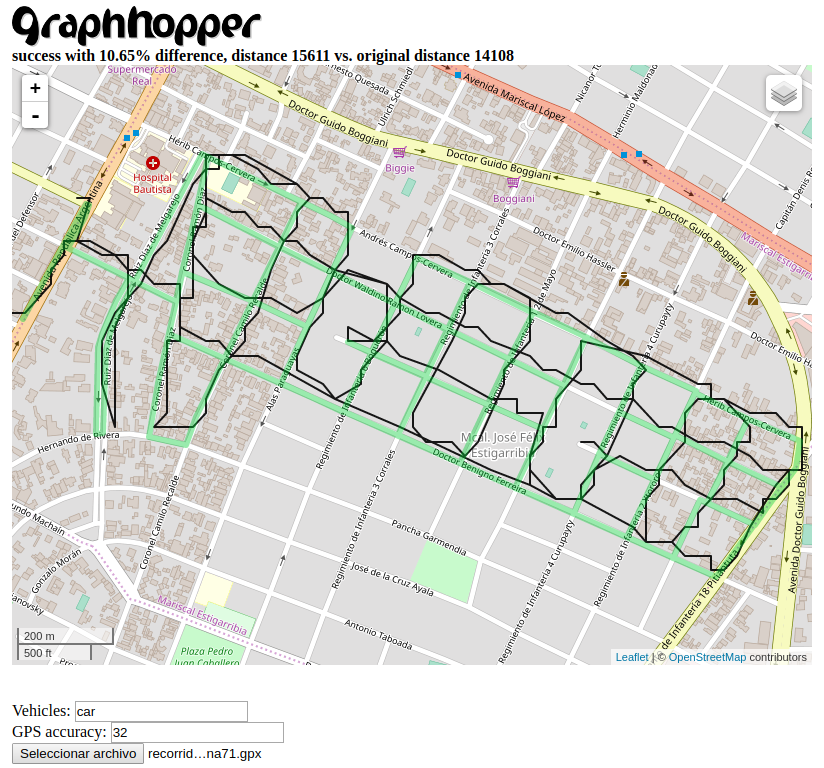
\includegraphics[width=\textwidth]{graphhopper71.png}
    \caption{Técnica \textit{Map Matching} aplicada sobre datos GPS de la DSU utilizando la herramienta \textit{open source} Graphhopper.}
    \label{fig:mapMatching}
\end{figure}

\begin{table}[tbp]
\caption{Comparación de resultados obtenidos con el actual.}
\label{table:comparacionActual}
\resizebox{\textwidth}{!}{%
\begin{tabular}{cccc}
\hline
Nombre de zona     & \begin{tabular}[c]{@{}c@{}}Distancia actual (km) \\ con Map matching\end{tabular} & Distancia generada (km) & \begin{tabular}[c]{@{}c@{}}Mejora con respecto \\ al actual (\%)\end{tabular} \\ \hline
71                 & \multirow{2}{*}{15.611}                                                           & 14.358                  & 8.02                                                                          \\
71 con opcionales  &                                                                                   & 13.320                  & 14.67                                                                         \\ \hline
3                  & \multirow{2}{*}{19.486}                                                           & 17.851                  & 8.39                                                                          \\
3 con opcionales   &                                                                                   & 16.879                  & 13.38                                                                         \\ \hline
119                & \multirow{2}{*}{16.940}                                                           & 14.704                  & 13.19                                                                         \\
119 con opcionales &                                                                                   & 13.825                  & 18.38                                                                         \\ \hline
21                 & \multirow{2}{*}{14.895}                                                           & 13.003                  & 12.7                                                                          \\
21 con opcionales  &                                                                                   & 11.675                  & 21.62                                                                         \\ \hline
22                 & \multirow{2}{*}{14.382}                                                           & 12.622                  & 12.24                                                                         \\
22 con opcionales  &                                                                                   & 11.635                  & 19.1                                                                          \\ \hline
83                 & \multirow{2}{*}{16.940}                                                           & 13.499                  & 20.31                                                                         \\
83 con opcionales  &                                                                                   & 12.112                  & 28.5                                                                          \\ \hline
\end{tabular}%
}
\end{table}

\section{Calidad de Software}

Existen varias definiciones para el concepto de Calidad de Software y la mayoría suele coincidir en la idea de adecuación a los requerimientos. La calidad de software está definida en \citet{Pressman2010IngenieriaPractico} como ``el proceso eficaz de software que se aplica de manera que crea un producto útil que proporciona valor medible a quienes lo producen y a quienes lo utilizan''. La ISO/IEC 9126 la define como ``el grado con el que un sistema, componente o proceso cumple los requerimientos especificados y las necesidades o expectativas del cliente o usuario''. 

Entre los atributos de la Calidad del Software tenemos: seguridad, fiabilidad, flexibilidad, robustez, comprensibilidad, testeabilidad, adaptabilidad, modularidad, complejidad, portababilidad, usabilidad, reusabilidad, eficiencia y facilidad.

A continuación se muestra un reporte con las métricas de algunos atributos de calidad en los proyectos \textit{backend} y \textit{frontend} de la aplicación. Las incidencias se fueron solucionando en ambos proyectos. (Ver Figuras \ref{fig:QAbackend}, \ref{fig:QAfrontend})

SonarQube define tres tipos de problemas:

\begin{itemize}
    \item \textit{Bug}: Un error de codificación que romperá su código y debe solucionarse de inmediato.
    \item \textit{Vulnerability}: Un punto en su código que está abierto al ataque.
    \item \textit{Code smell}: Un problema de mantenibilidad que hace que su código sea confuso y difícil de mantener.
\end{itemize}

Cada problema corresponde a una de las cinco severidades:

\begin{itemize}
    \item \textit{Blocker}: Error con una alta probabilidad de afectar el comportamiento de la aplicación en producción: pérdida de memoria, conexión JDBC no cerrada, etc. El código debe ser arreglado de inmediato.
    \item \textit{Critical}: Ya sea un error con poca probabilidad de afectar el comportamiento de la aplicación en producción o un problema que representa un defecto de seguridad: bloque de captura vacío, inyección de SQL, etc. El código debe revisarse de inmediato.
    \item \textit{Major}: Defecto de calidad que puede tener un gran impacto en la productividad del desarrollador: pieza de código descubierta, bloques duplicados, parámetros no utilizados.
    \item \textit{Minor}: Defecto de calidad que puede afectar ligeramente la productividad del desarrollador: las líneas no deben ser demasiado largas, las declaraciones de "cambio" deben tener al menos 3 casos, entre otros.
    \item \textit{Info}: Ni un error ni un defecto de calidad, solo un hallazgo.
\end{itemize}

\begin{figure}[htbp]
    \centering
    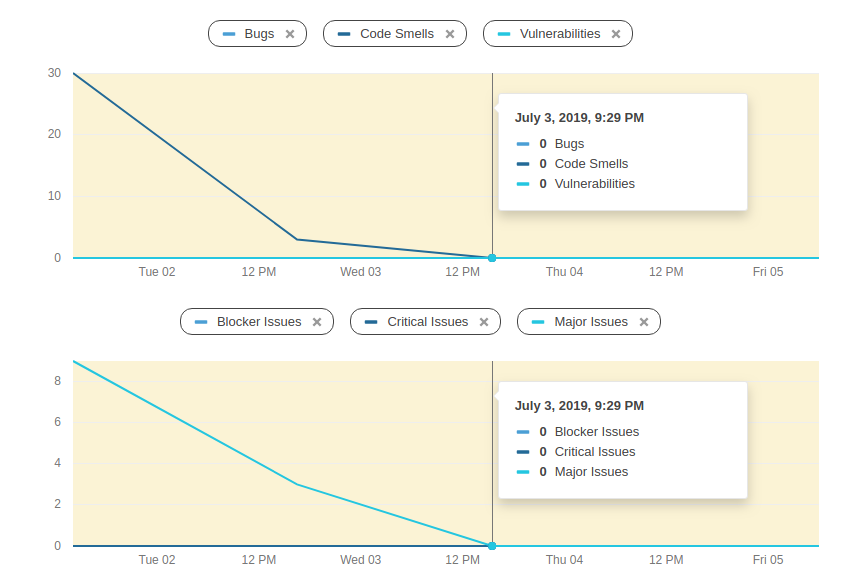
\includegraphics[width=\textwidth]{reporteQA_BE.png}
    \caption{Reporte de inspección de código con SonarQube del \textit{Backend}.}
    \label{fig:QAbackend}
\end{figure}

\begin{figure}[htbp]
    \centering
    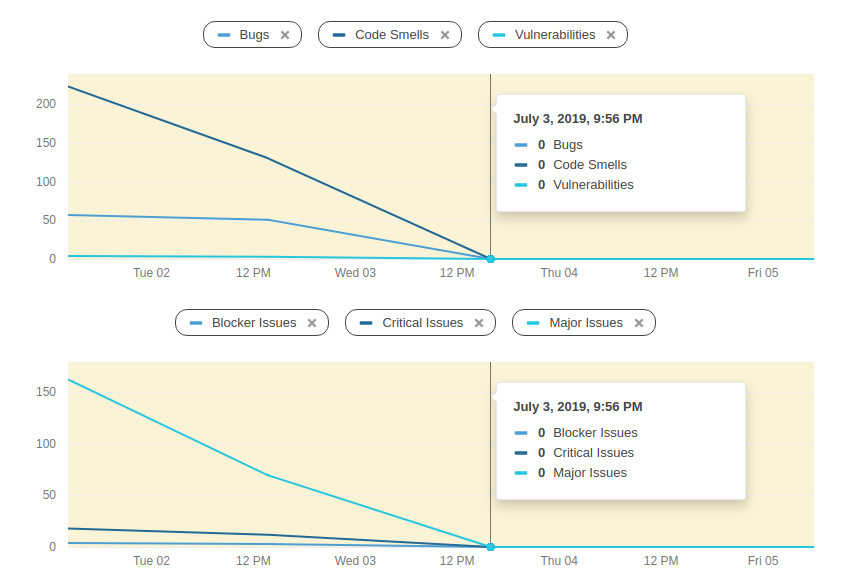
\includegraphics[width=\textwidth]{reporteQA_FE2.png}
    \caption{Reporte de inspección de código con SonarQube del \textit{Frontend}.}
    \label{fig:QAfrontend}
\end{figure}

% \subsection{Usabilidad}